\documentclass[12pt]{article}
\usepackage[english]{babel}
\usepackage[utf8]{inputenc}

\usepackage{geometry}
\geometry{
	letterpaper, 
	portrait, 
	top=.75in,
	left=.8in,
	right=.75in,
	bottom=.5in		} 	% Page Margins
	
%% additional packages for nice things
\usepackage{amsmath} 	% for most math
\usepackage{commath} 	% for abs
\usepackage{lastpage}	% for page count
\usepackage{amssymb} 	% for therefore
\usepackage{graphicx} 	% for image handling
\usepackage{wrapfig} 	% wrap figures
\usepackage[none]{hyphenat} % for no hyphenations
\usepackage{booktabs} 	% enhanced table qualities
\usepackage{array} 		% for >{} column characterisctis
\usepackage{physics} 	% for easier derivative \dv....
\usepackage{tikz} 		% for graphic@!
\usepackage{circuitikz} % for circuits!
\usetikzlibrary{arrows.meta} % for loads
\usepackage[thicklines]{cancel}	% for cancels
\usepackage{xcolor}		% for color cancels
\usepackage[per-mode=fraction]{siunitx} % for si units and num
\usepackage{fancyhdr} 	% for header
\usepackage{comment}	% for ability to comment out large sections
\usepackage{multicol}	% for multiple columns using multicols
\usepackage[framed,numbered]{matlab-prettifier} % matlab sytle listing
\usepackage{marvosym} 	% for boltsymbol lightning
\usepackage{pdflscape} 	% for various landscape pages in portrait docs.
\usepackage{float}
\usepackage{fancyvrb}	% for Verbatim (a tab respecting verbatim)
\usepackage{enumitem}	% for [resume] functionality of enumerate

%% package config 
\sisetup{output-exponent-marker=\ensuremath{\mathrm{E}}} % for engineer E
\renewcommand{\CancelColor}{\color{red}}	% for color cancels
\lstset{aboveskip=2pt,belowskip=2pt} % for more compact table
\def\arraystretch{1.4} % adjust size of arrays
%\arraycolsep=1.4pt\def
\setlength{\parindent}{0cm} % Remove indentation from paragraphs
\setlength{\columnsep}{0.5cm}
\lstset{
	style      = Matlab-editor,
	basicstyle = \ttfamily\footnotesize, % if you want to use Courier - not really used?
}
\renewcommand*{\pd}[3][]{\ensuremath{\dfrac{\partial^{#1} #2}{\partial #3}}} % for larger pd fracs
\renewcommand{\real}[1]{\mathbb{R}\left\{ #1 \right\}}	% for REAL symbol
\newcommand{\imag}[1]{\mathbb{I}\left\{ #1 \right\}}	% for IMAG symbol
\definecolor{m}{rgb}{1,0,1}	% for MATLAB matching magenta
	
%% custom macros
\newcommand\numberthis{\addtocounter{equation}{1}\tag{\theequation}} % for simple \numberthis command
\newcommand{\equal}{=} % so circuitikz can have an = in the labels
\newcolumntype{L}[1]{>{\raggedright\let\newline\\\arraybackslash\hspace{0pt}}m{#1}}
\newcolumntype{C}[1]{>{\centering\let\newline\\\arraybackslash\hspace{0pt}}m{#1}}
\newcolumntype{R}[1]{>{\raggedleft\let\newline\\\arraybackslash\hspace{0pt}}m{#1}}

%% Header
\pagestyle{fancy} % for header stuffs
\fancyhf{}
\rhead{Thad Haines \\ Page \thepage\ of \pageref{LastPage}}
\chead{Talking Points \\ Week of April 8, 2019}
\lhead{Research \\ }
% spacing
\headheight 29 pt
\headsep 6 pt

\begin{document}
\begin{multicols}{2}

	\paragraph{Recent Progress:}
	\begin{enumerate}
		\item Python ODE solver utilized for system frequency calculation (runge kutta 45)

		\item tgov1 model created and validated via steps and ramps of PSLF ee544 system.
		
		\item More \verb|matplotlib| plot functions created.

		\item GitHub updated:\\
		\verb|https://github.com/thadhaines/PSLTDSim/|
		
	\end{enumerate}
\paragraph{Current Tasks:}
	\begin{enumerate}
	
		\item Begin parsing WECC dyd and address associated code issues that arise.

		\item Formulate feasible plan of action for casting WECC governors to LTD governors.
		
		\item Create an agent for every object: Shunt, SVD, Branch, Transformer, ...

		\item Define Agent actions for \\ AGC/LFC (i.e. ACE calculations)

		\item Formulate an experiment utilizing a multi-area model that can be validated with PSLF.

		\item Investigate line current data and ULTC action in PSLF.

		
		%\subitem A FlowtabrDAO exists that can find flow between busses. A way to initialize bus connections between areas has yet to be devised.
		

	\end{enumerate}
%\pagebreak
\vfill\null
\columnbreak

\paragraph{Future Tasks:}(Little to No Progress since last time / Things coming down the pipe)
	\begin{enumerate}
		\item Think about Shunt Control / Generic Agent control based on system state(s)

		\item Flow chart AMQP process to more clearly explain what's happening there/ find possible speed improvements.

		\item Identify System Slack bus programmatically (currently assumes first slack if > 1)
		\subitem AND/OR calculate system slack error differently $\rightarrow$ An average of slack errors?

		\item Matt request: Enable multiple dyd files to overwrite / replace previously defined agents/parameters
		
		%\subitem Can locate when only 1 Slack exists. If more than one Slack, maybe identify by generator with most busses under control? Proving more difficult than expected. Can identify in PSLF via the \verb|summ()| or \verb|isld()| commands. 
		
	\end{enumerate}
	\paragraph{Current Questions:}
	\begin{enumerate}
		
		\item Overview of planned PSLF scenarios? $\rightarrow$ Similar to Heredia paper but on Wecc/MiniWecc Scale? Yes.
		
		\item Is there more available/relevant event data that may help us to verify simulations of specific instances (wind ramps or other behavior) that novel research will focus on?\\ (Heredia paper data helpful for some wind ramp data context)

		\item  Any progress / continued interest in miniWecc Area definitions?

		\item Any progress on Wecc single gen per bus system?
		\\ Will this actually matter? PSLF handles distribution of Pe in power flow solution per bus, and LTD code distributes electrical power per generator... Voltage issues feel probable...
		
		
%		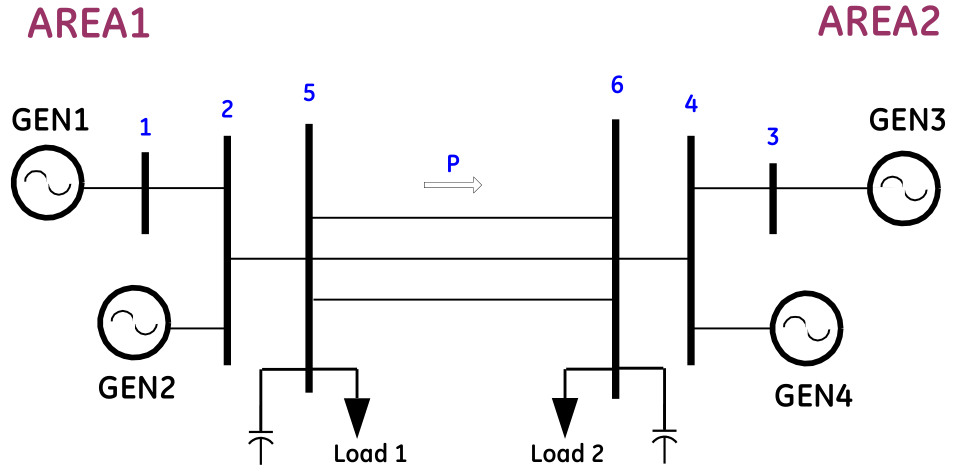
\includegraphics[width=\linewidth]{g4aSys}
	\end{enumerate}

\vfill\null

\end{multicols}
	\begin{comment}
\pagebreak

\begin{landscape}
\begin{centering}
%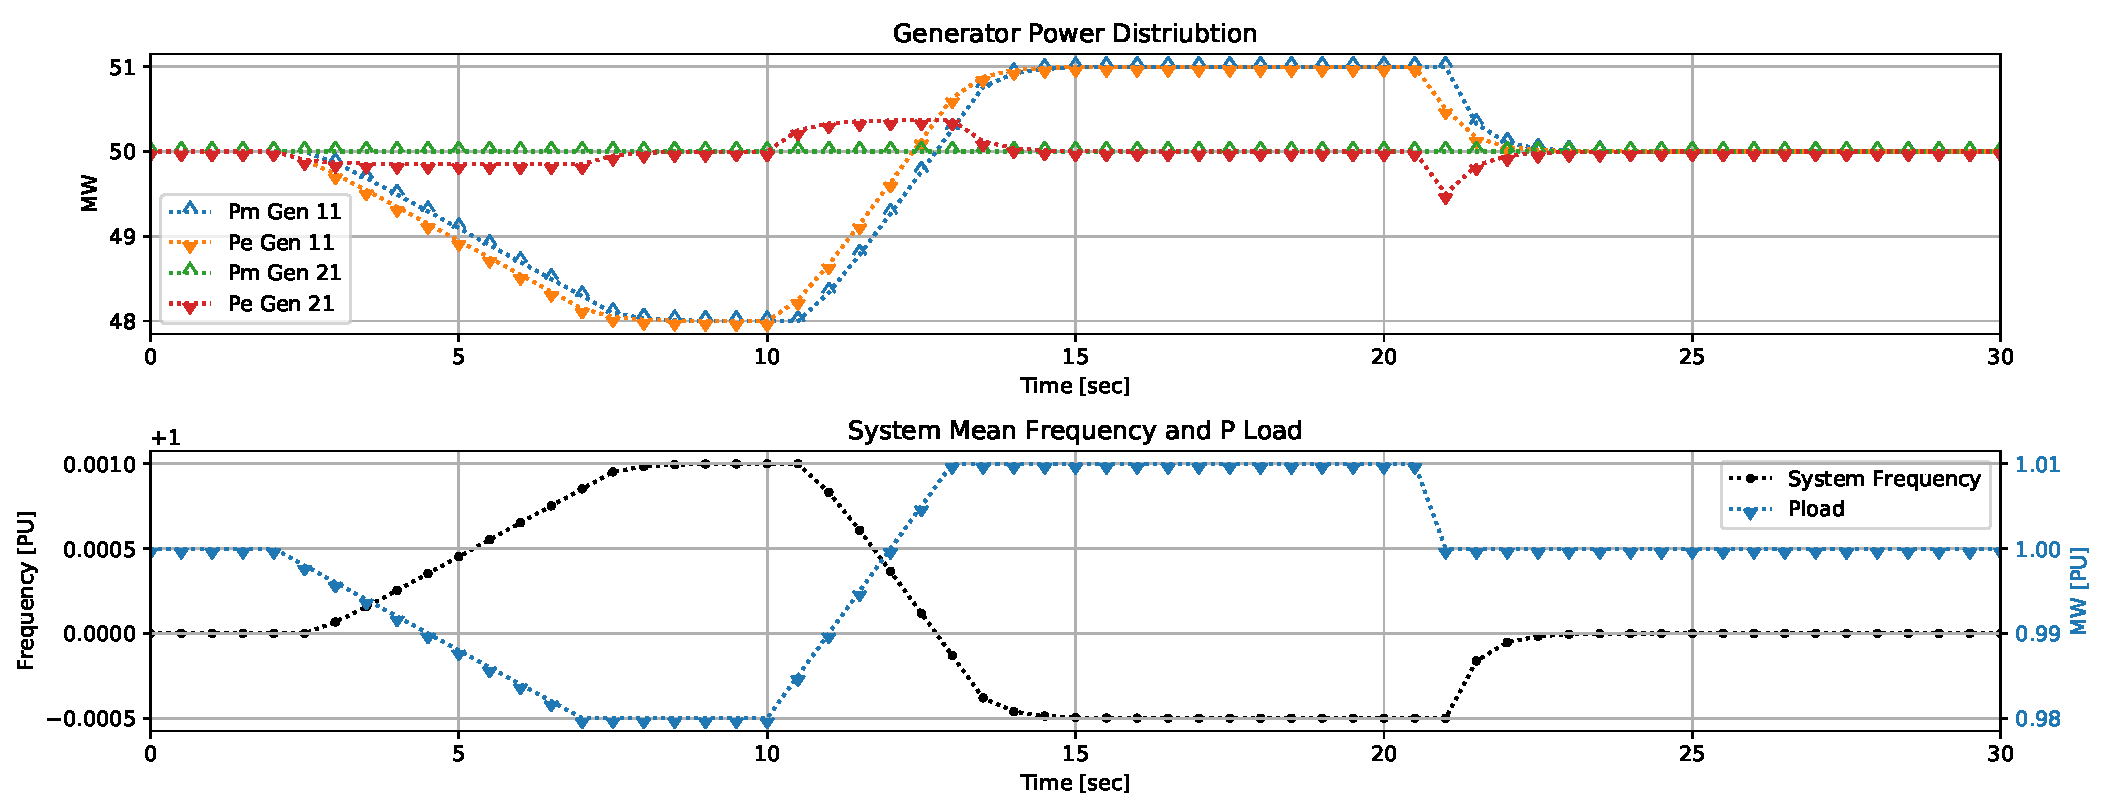
\includegraphics[width=\linewidth]{pythonRamp02}
\vspace{-1em}
\end{centering}
\vspace{-1em}
\paragraph{.ltd File Example:}
\begin{Verbatim}
# LTD simulation models / perturbances 
# Commented and empty lines are ignored during parsing.
# Double quoted variable names in model parameters also ignored

# pgov1  busnum busnam basekv id : #9 mwcap droop k1
#pgov1   21 "21" 22.00 "1 " : #9 mwcap=100.0 "droop" 0.05 "k1" 1.0
pgov1   11 "11" 22.00 "1 " : #9 mwcap=100.0 0.05 1.0

# Perturbances
# target bus id(optional) : pertType attribute time val abs(optional)
load 3 : "pertType" step  "pertTarget" p "startTime" 21 "newVal" -1 rel
load 3 : "pertType" ramp "pertTarget" p "startTime" 2 "RAtime" 5 "RAval" -2 "holdtime" 3 "RBtime" 3 "RBval" 3
\end{Verbatim}
\end{landscape}

 	place for comments

	\end{comment}
\end{document}